\begin{figure}
	\centering
	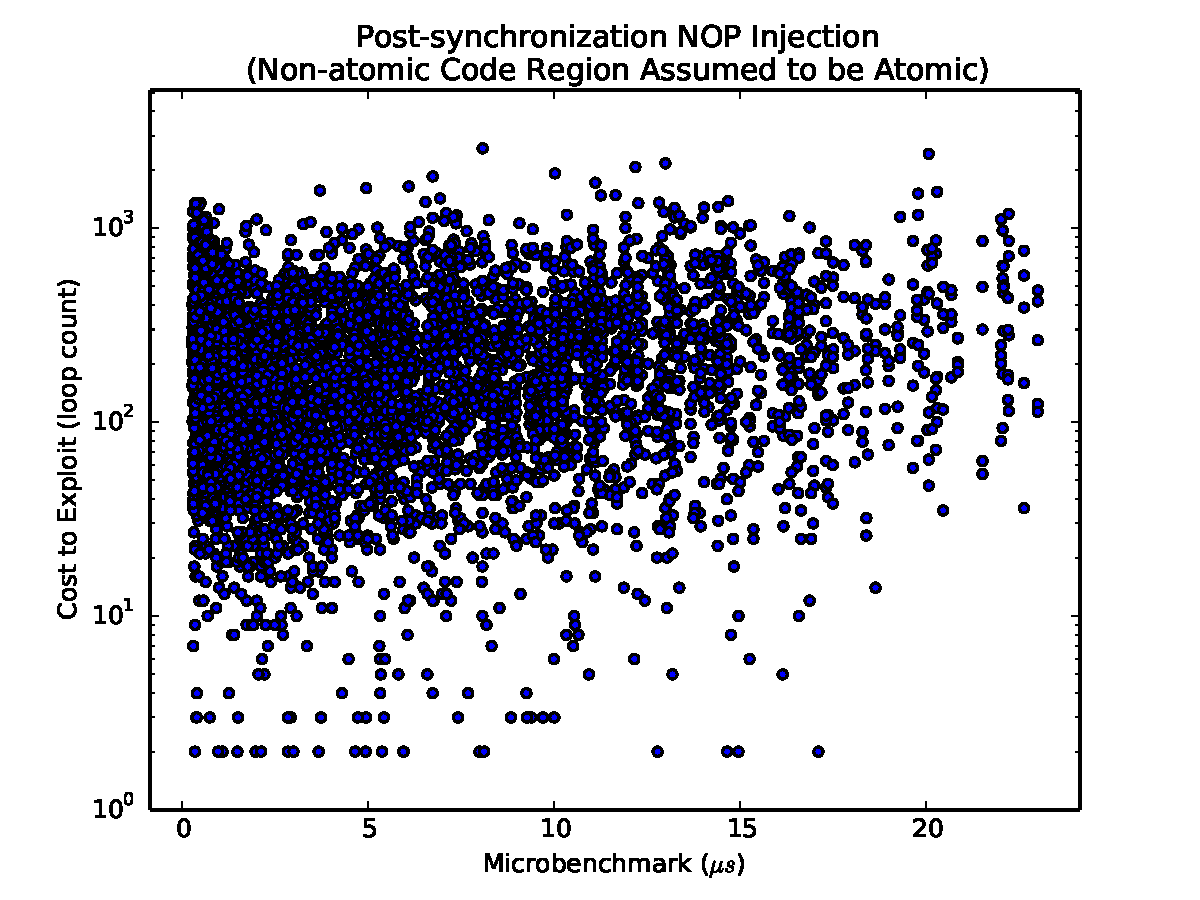
\includegraphics[width=\columnwidth]{figures/nonatomic-post}
	\caption{Exploit cost (in number of exploit attempts) as a function of the microbenchmark after applying diversity implementation 3 to a canonical "nonatomic-region-assumed-to-be-atomic" concurrency bug.}
	\label{fig_nonatomic-post}
\end{figure}

\begin{figure}
	\centering
	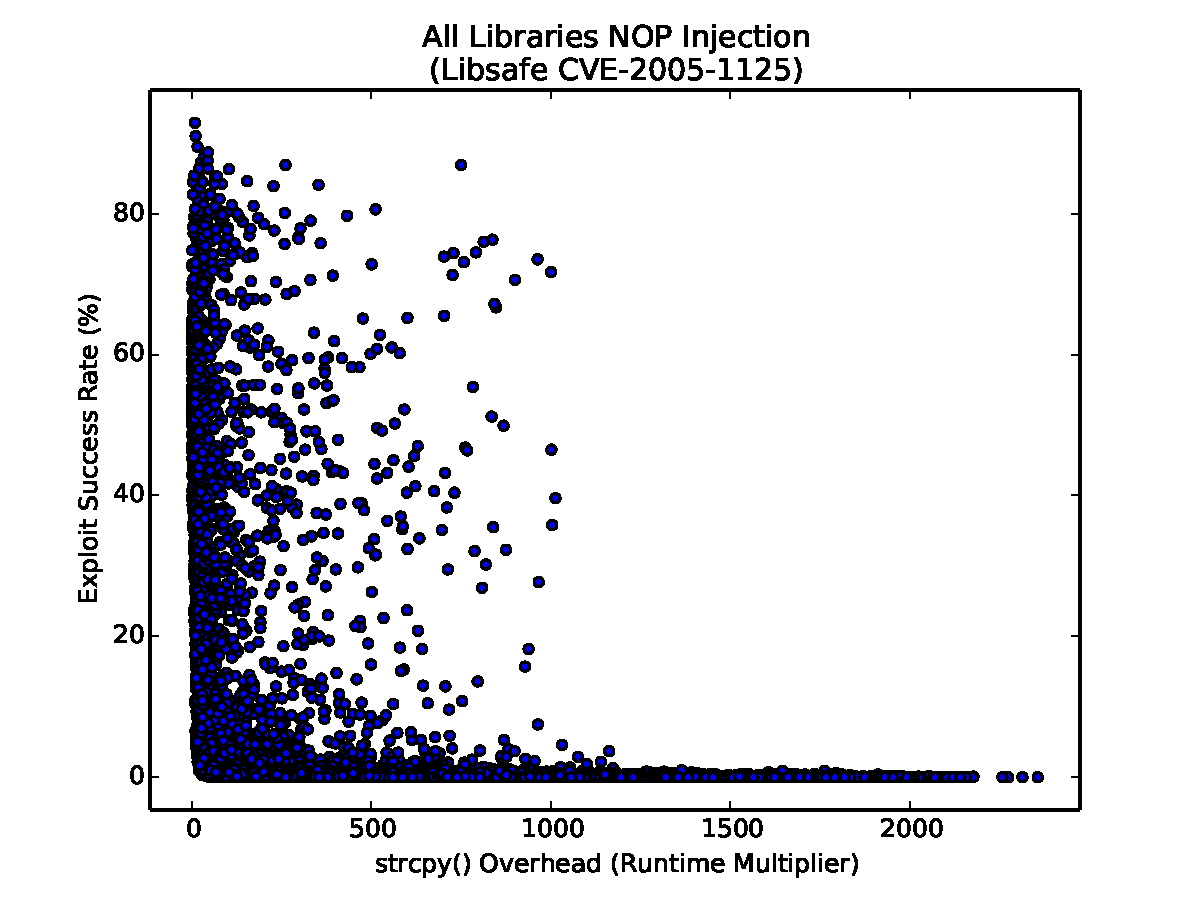
\includegraphics[width=\columnwidth]{figures/libsafe-all}
	\caption{Exploit success rate as a function of the microbenchmark after applying diversity implementation 1 to Libsafe with concurrency bug CVE-2005-1125.}
	\label{fig_libsafe-all}
\end{figure}

\begin{figure}
	\centering
	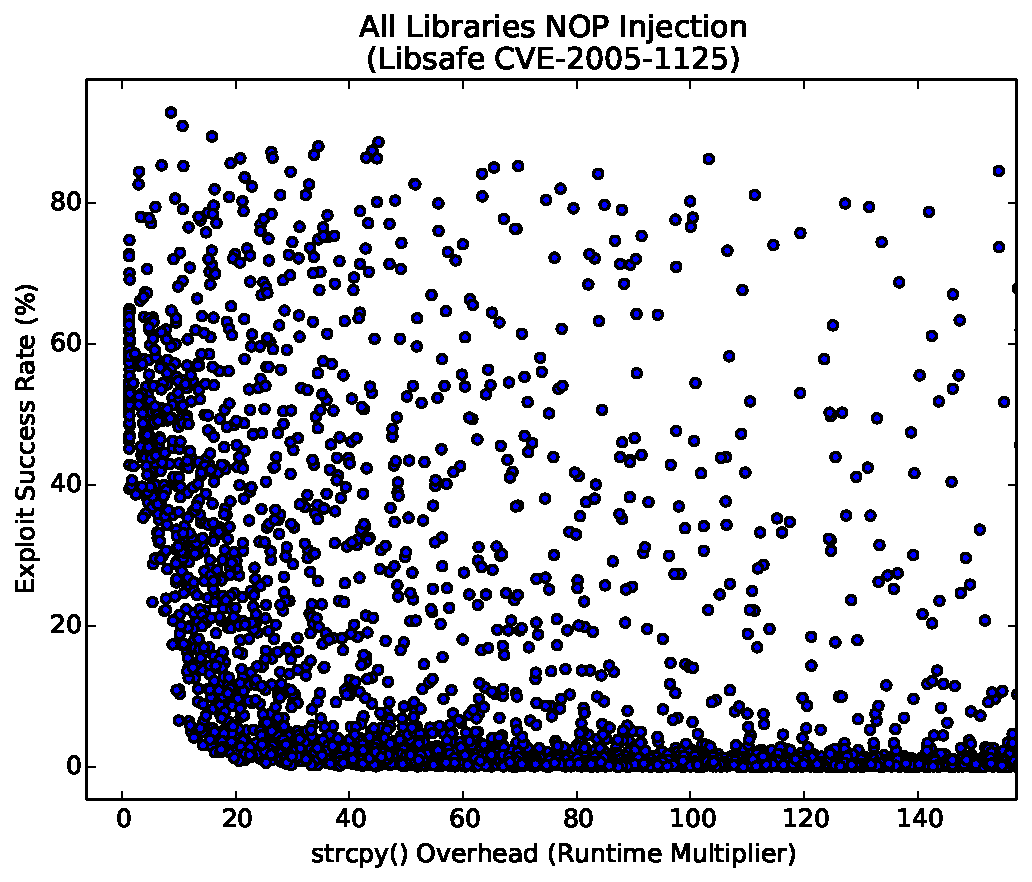
\includegraphics[width=\columnwidth]{figures/libsafe-all-zoom}
	\caption{Exploit success rate as a function of the microbenchmark after applying diversity implementation 1 to Libsafe with concurrency bug CVE-2005-1125 (a zoom-in of Figure \ref{fig_libsafe-all}).}
	\label{fig_libsafe-all-zoom}
\end{figure}

\begin{figure}
	\centering
	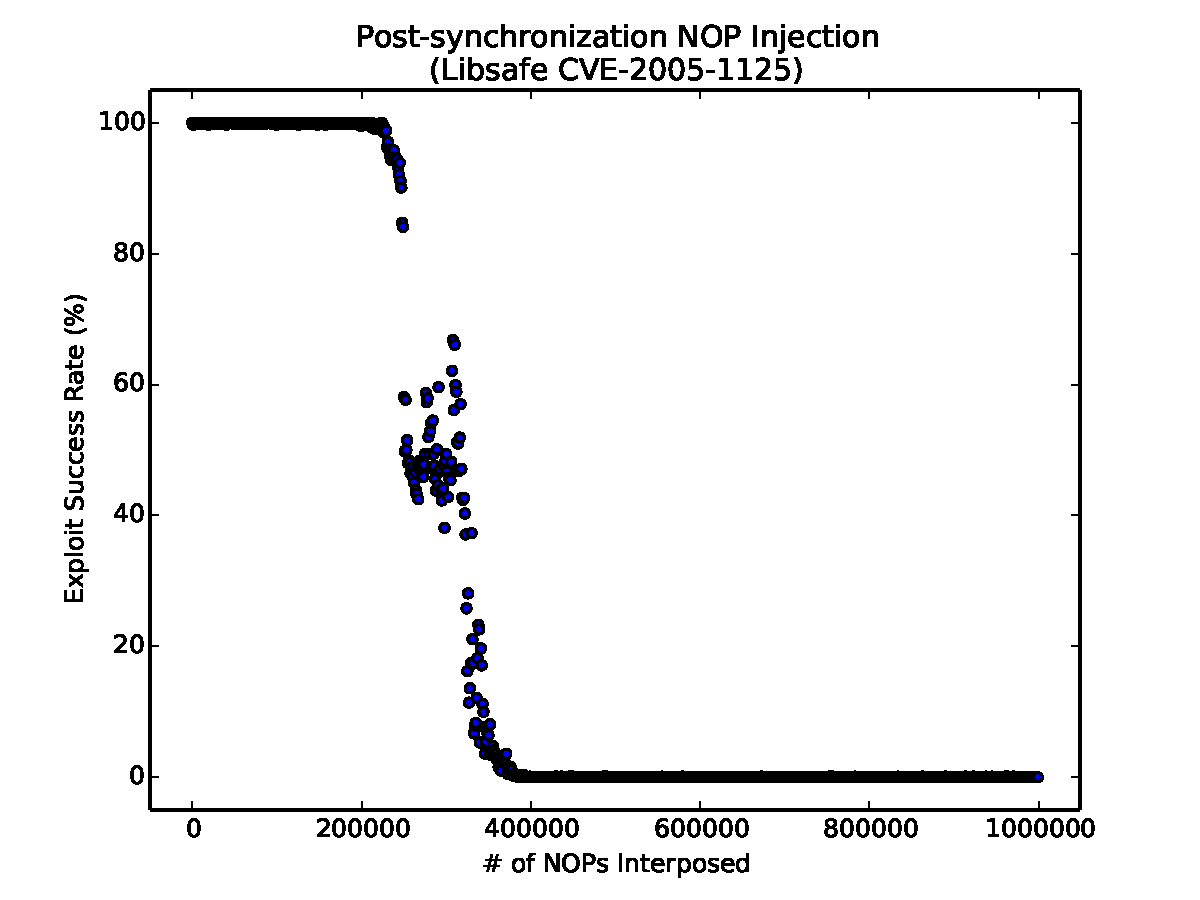
\includegraphics[width=\columnwidth]{figures/libsafe-post}
	\caption{Exploit success rate as a function of the number of NOPs injected after applying diversity implementation 3 to Libsafe with concurrency bug CVE-2005-1125.}
	\label{fig_libsafe-post}
\end{figure}

\begin{figure}
	\centering
	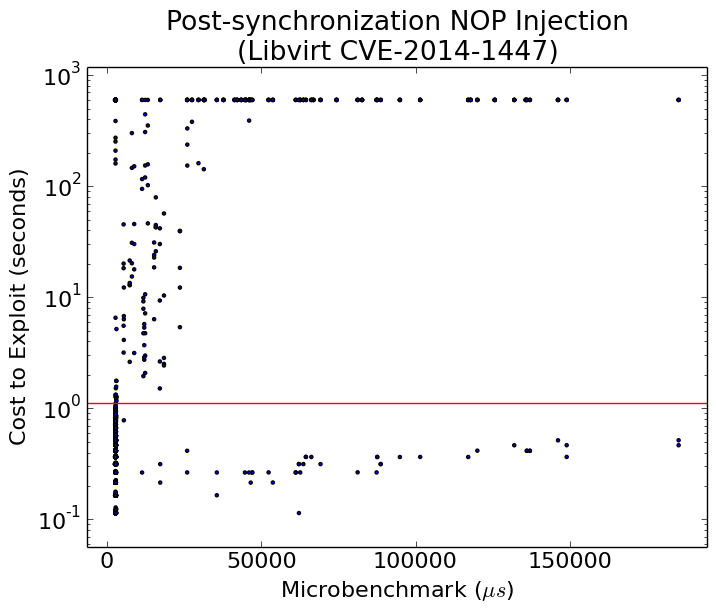
\includegraphics[width=\columnwidth]{figures/libvirt-post}
\caption{Exploit cost (in time) as a function of the microbenchmark after applying diversity implementation 3 to Libvirt with concurrency bug CVE-2014-1447.}
	\label{fig_libvirt-post}
\end{figure}